\chapter{Systembeskrivelse}
Dette kapitel indeholder en introducerende beskrivelse af den udviklede prototype, herunder brugergrænsefladen og dens fysiske opbygning. Herudover indeholder kapitlet en beskrivelse af sorteringsprocessen og generelle egenskaber for de langerhanske øer.

Figur \ref{fig:system} viser den overordnede opbygning af systemet. Grundlæggende består systemet af en beholder indeholdene opløsningen med langerhanske øer. Opløsningen pumpes herefter ved hjælp af en pumpe i gennem en slange, hvor et kamera detektere om en ø passere eller ej. Hvis en ø detekteres åbner systemet en ventil for at frasortere øen fra resten af opløsningen. Systemet består af et software program udviklet i Matlab, hvor operatøren har mulighed for at interagere med systemet. Her er selve logikken og signalbehandlingen i form af billedprocessering implementeret. Programmet giver signal til en Microcontroller (Arduino platform), som håndterer den videre styring af hardware komponenterne.

\begin{figure}[H]
	\centering
	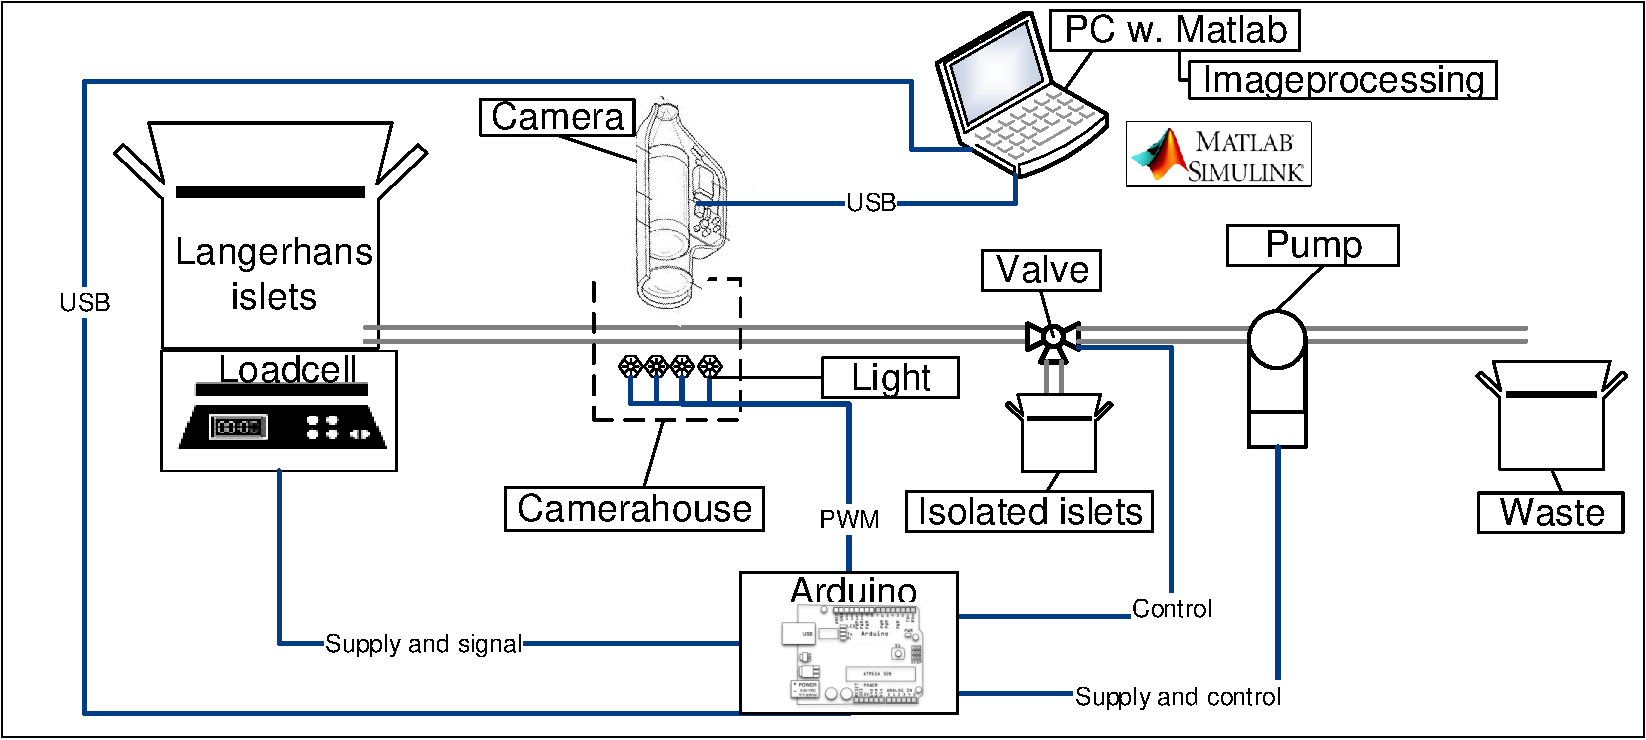
\includegraphics[width=1\textwidth]{billeder/DMTS.pdf}
	\caption{Figuren viser den overordnede opbygning af systemet}
	\label{fig:system}
\end{figure}
%Beskrivelse 
%
%Figur over systemet
%
%Billeder af det færdige system


\section{Brugergrænseflade}
Skal brugergrænseflade og hardware først komme i resultat afsnittet XX 

Billeder og beskrivelser

\section{Hardware}
Skal brugergrænseflade og hardware først komme i resultat afsnittet XX 

\section{Sorteringsproces}
Dette afsnit beskriver hvordan sorteringsprocessen foregår, samt generelle egenskaber for opløsningen med langerhanske øer. 

\subsection{Sorteringsproces} \label{subsec:sortproces} \fxnote{Vi venter stadig på den faktiske protokol fra SG}
Som det kort blev beskrevet i baggrundsafsnittet består isoleringen af langerhanske øer af 3 faser. 
Figur \ref{fig:sortproces} viser den trinvise proces fra intakt pankreas til isoleret ø.

\begin{figure}[H]
	\centering
	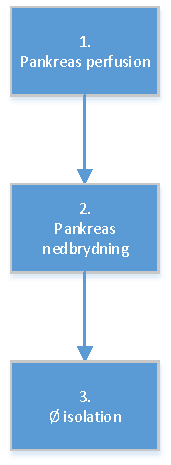
\includegraphics[width=0.2\textwidth]{billeder/sortering-crop.pdf}
	\caption{Sorteringsproces}
	\label{fig:sortproces}
\end{figure}

Den første fase, \textit{pankreas perfusionen}, foregår ved at man først operativt fjerner pancreas, hvorefter enzymet collagenase sprøjtes ind i pankreas. Dette enzym starter en nedbrydning af vævet i pankreas. Enzymet har den egenskab, at det ikke nedbryder de langerhanske øer, men derimod kun det omkringliggende væv.

I anden fase, \textit{pankreas nedbrydningen}, nedbrydes pankreasen yderligere ved at den bliver skåret i mindre dele og pankreas placeres i en inkubator ved 37,5 grader. Dette gøres for at accelerere nedbrydningen af pankreas. Når pankreas er nedbrudt nedkøles vævet for, at stoppe virkningen af collagenase. 

I den sidste fase, \textit{ø isolation}, bliver øerne frasorteret fra det omkringliggende væv. 


\subsection{Langerhanske øer}
Den endelige opløsning består udover de langerhanske øer af ekstra væv fra pankreas og fysiologisk saltvand.

Figur \ref{fig:islet}, viser hvordan opløsningen ser ud. På billedet er opløsningen hældt i en petriskål.

\begin{figure}[H]
	\centering
	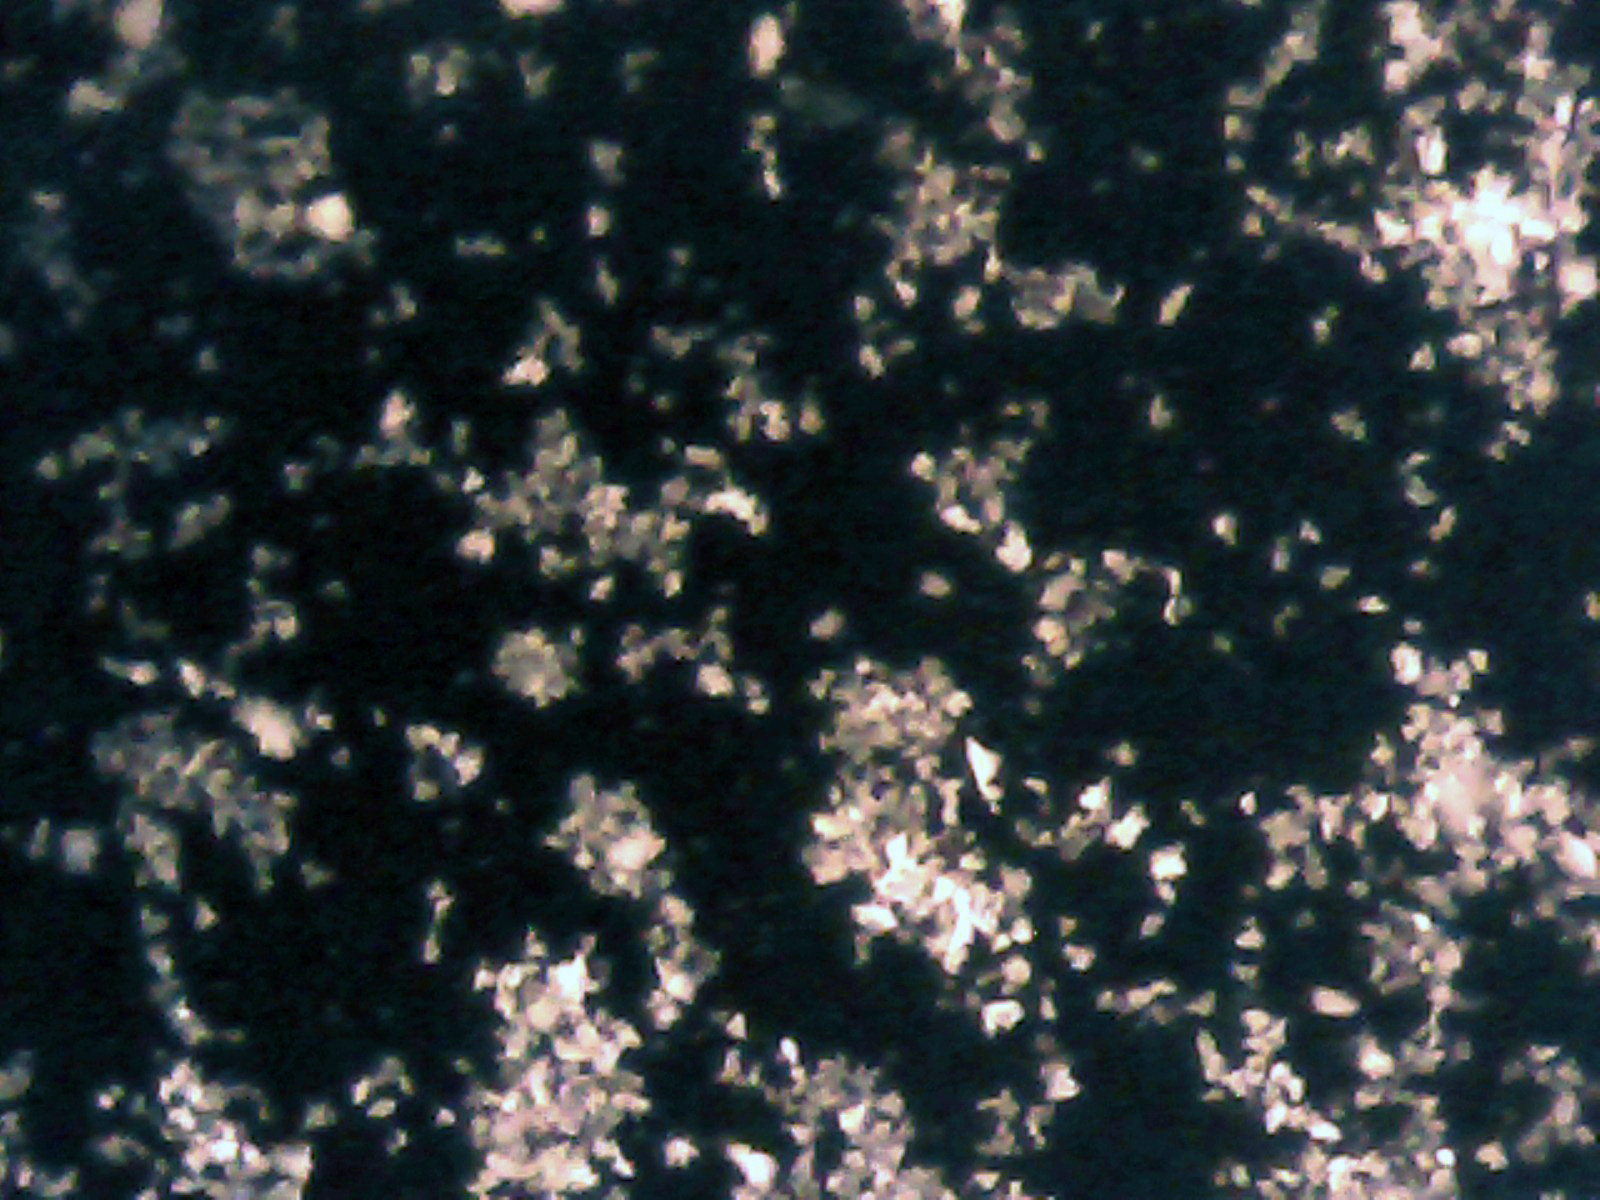
\includegraphics[width=0.5\textwidth]{billeder/software/2.jpg}
	\caption{Opløsning med langerhanske øer}
	\label{fig:islet}
\end{figure}

En petriskål på 10 ml vil typisk indeholde mellem 30 og 50 øer. Til et batch på 250 øer anvnedes typisk 5-6 mus. Den samlede mængde opløsningsvæske i sådan et batch er 250 ml.. (vi mangler at få konkrete tal fra SG)

Øerne har en størrelse mellem 100 og 300 um.





